\section{Durchführung}

\subsection{Bau des Roboterarmes}
\schritt{1}{Den Roboterarm vorbereiten}{
Die Pappe schneidet ihr in sechs 30cm lange und 2cm breite Streifen. Davon halbiert ihr zwei, sodass ihr vier 15cm lange Streifen habt. Zwei von diesen kürzt ihr nochmal auf 12cm.\\

Außerdem benötigt ihr vier Pappteile, die ihr wie auf dem Bild zuschneidet, zirka 12 kleine Pappquadrate und zwei Pappkreise, deren Durchmesser ungefähr mit der Größe der Reifen übereinstimmt.\\

Die Pappstreifen werden jetzt zusammengeklebt.
Dafür klebt ihr jeweils zwei gleichlangen Streifen mit Heißkleber zusammen, sodass ihr zwei 30cm, ein 15cm und ein 12cm langes Pappstück habt.\\

Die vier Pappteile klebt ihr übereinander zu einem Klotz. An diesem können später die Stifte mit der Maulklemme befestigt werden.\\

}

\begin{figure}[h]
\centering
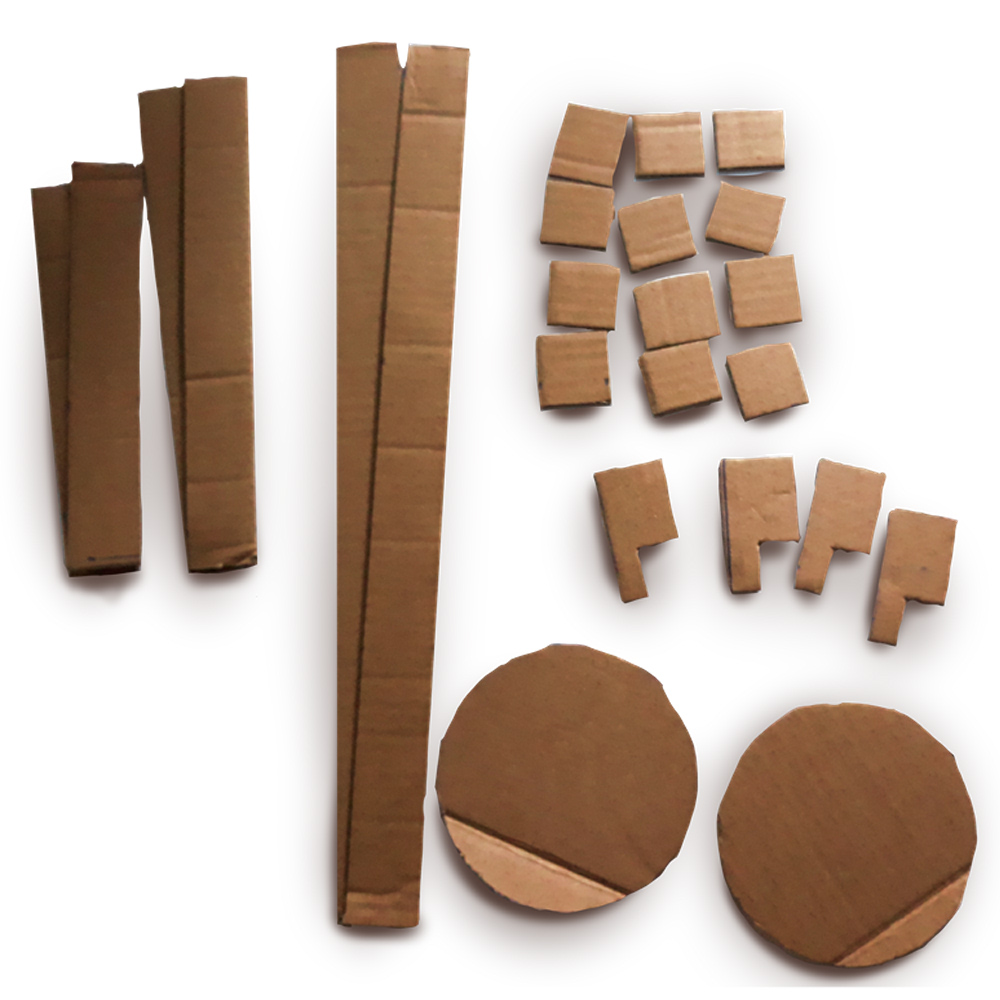
\includegraphics[width=5cm]{pappstucke.jpg}
\caption*{Stifte}
\end{figure}

\schritt{2}{Den Roboterarm bauen}{
Die Pappteile müssen zu einem Arm zusammengebaut werden. Dabei bilden zwei kleine Pappquadrae und ein Zahnstocher ein Gelenk, das die Pappteile miteinander verbindet.
Am besten orientiert ihr euch an der folgenden Grafik:\\


Falls ihr nicht weiterwisst, gibt es auch eine ausführlichere Beschreibung auf https://tuduu.org/projekt/automatischer-malroboter .\\
Den Pappblock klebt ihr auf die Unterseite des Arms, also nicht die Fläche, auf welcher der zweite Pappstreifen aufliegt.\\

Wenn alles zusammengesteckt und verbunden ist, testet euren Arm vorsichtig. Bewegt sich alles reibungslos?\\

Dann verklebt die Zahnstocher zum Schluss oben und unten mit einem Tropfen Heißkleber, dann hällt alles ein bisschen besser.\\
Die Pappkreise klebt ihr so auf die Reifen, dass die Pappstreifen oben auf liegen.\\

}
\begin{figure}[h]
\centering
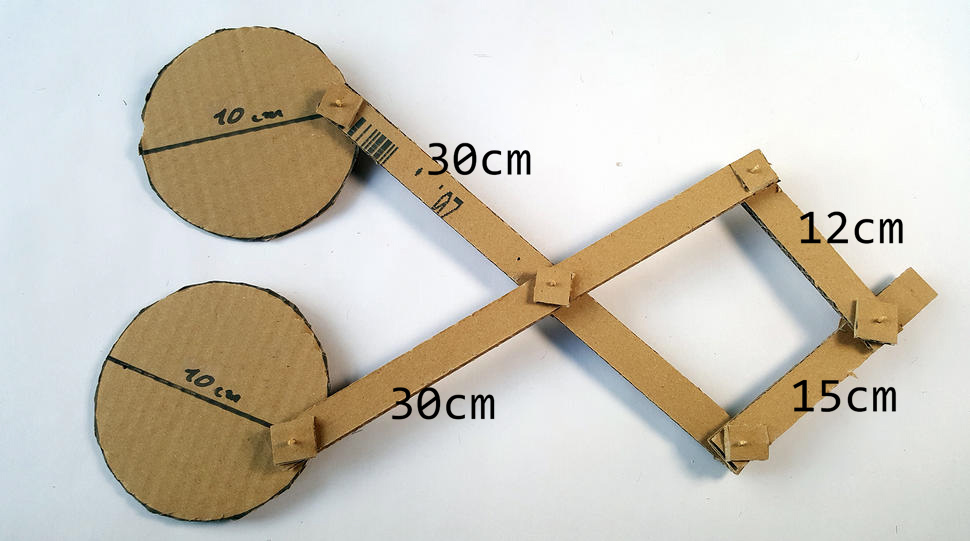
\includegraphics[width=5cm]{arm.jpg}
\caption*{Der Roboterarm sollte sich reibungslos bewegen lassen}
\end{figure}



\subsection{Verbindung mit RaspberryPi}

\begin{center}
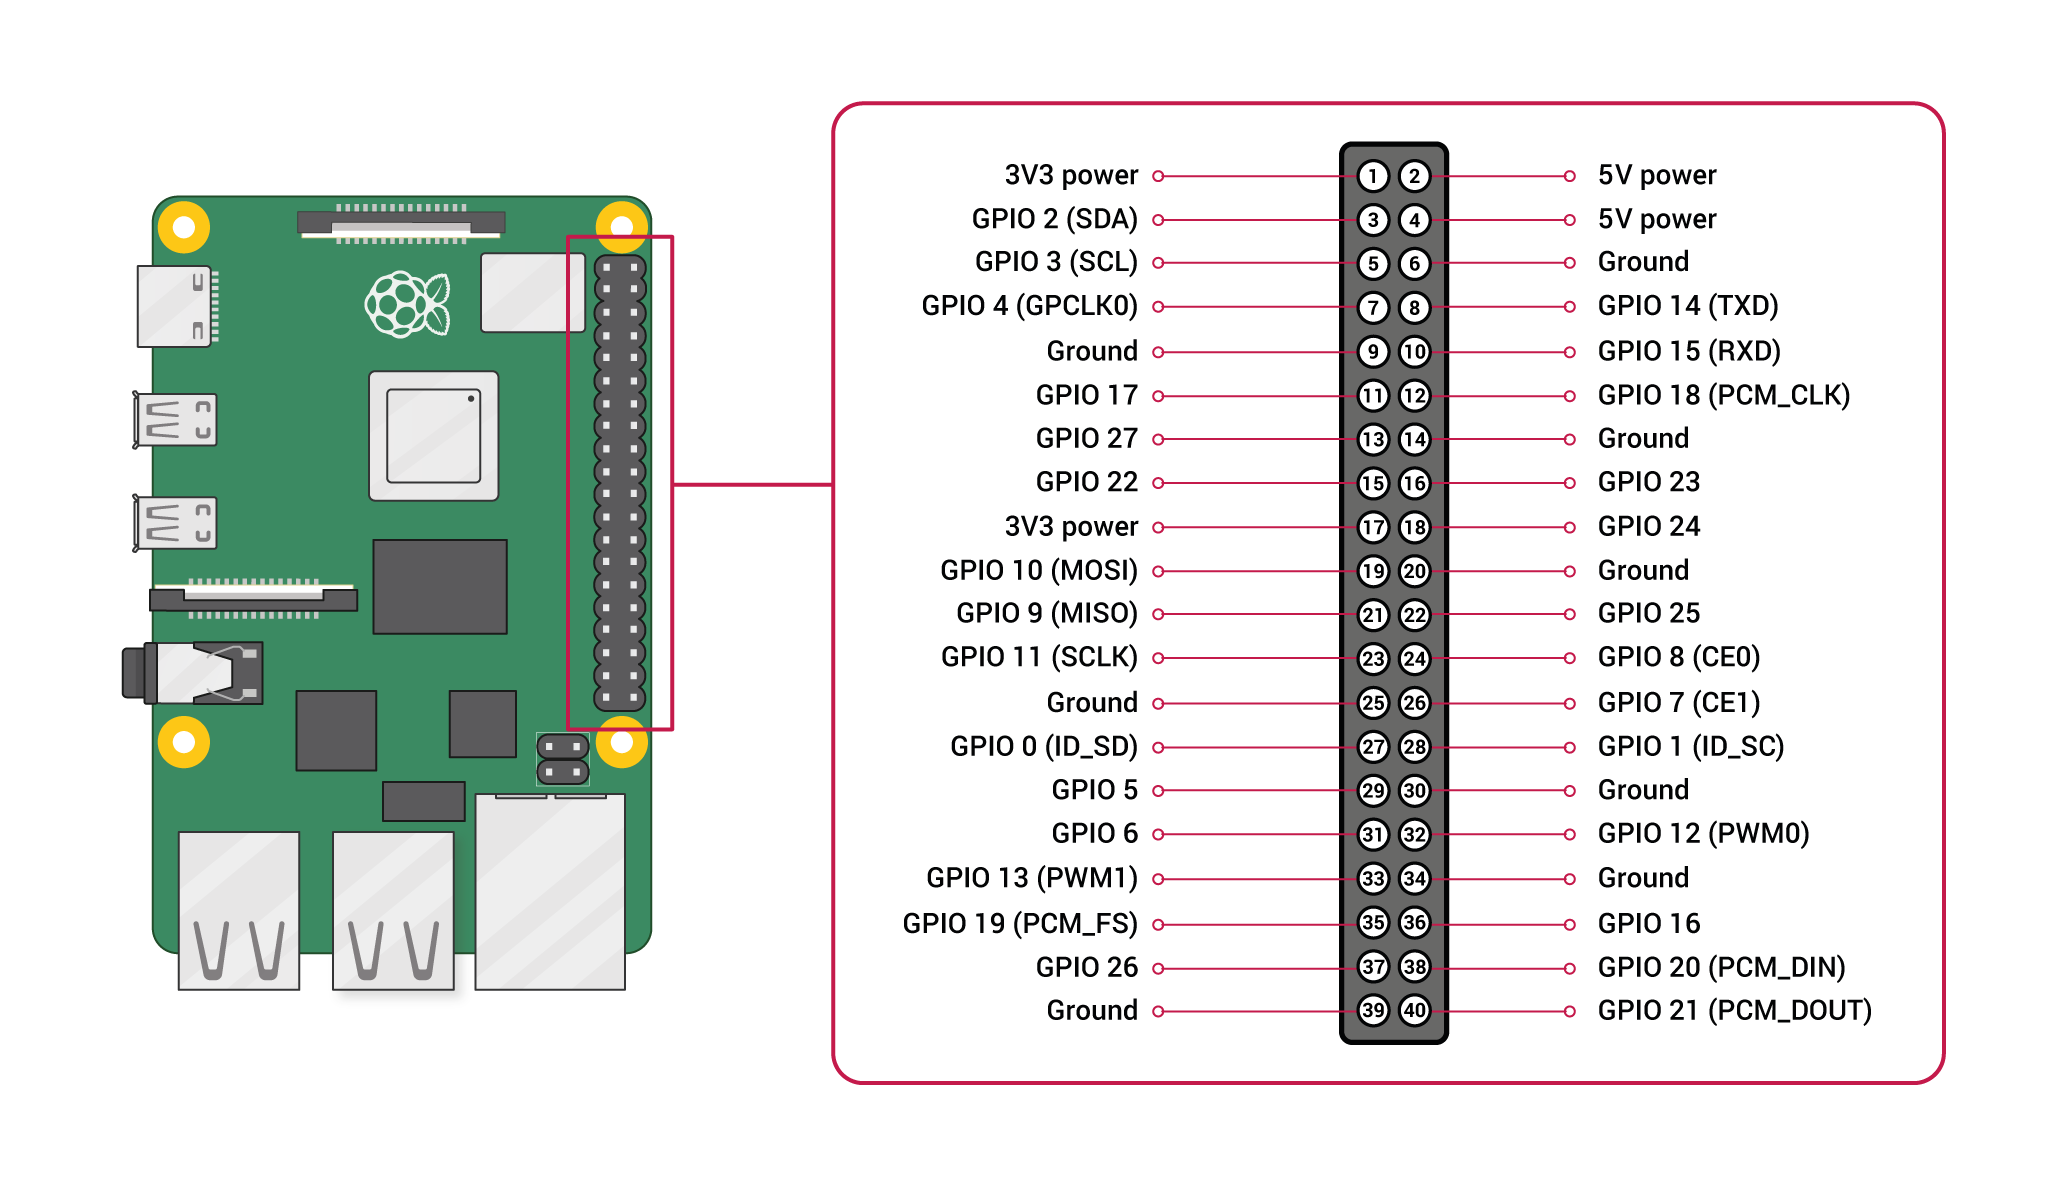
\includegraphics[width=\textwidth]{rpi_gpio_pinout.png}
\end{center}

\begin{figure}[h]
\centering
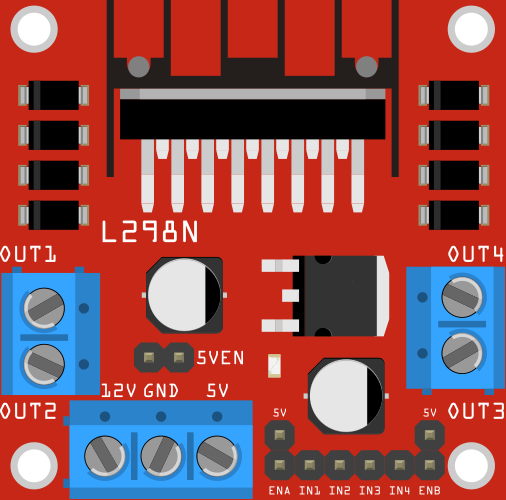
\includegraphics[width=5cm]{l298n.png}
\end{figure}

\begin{figure}[h]
\centering
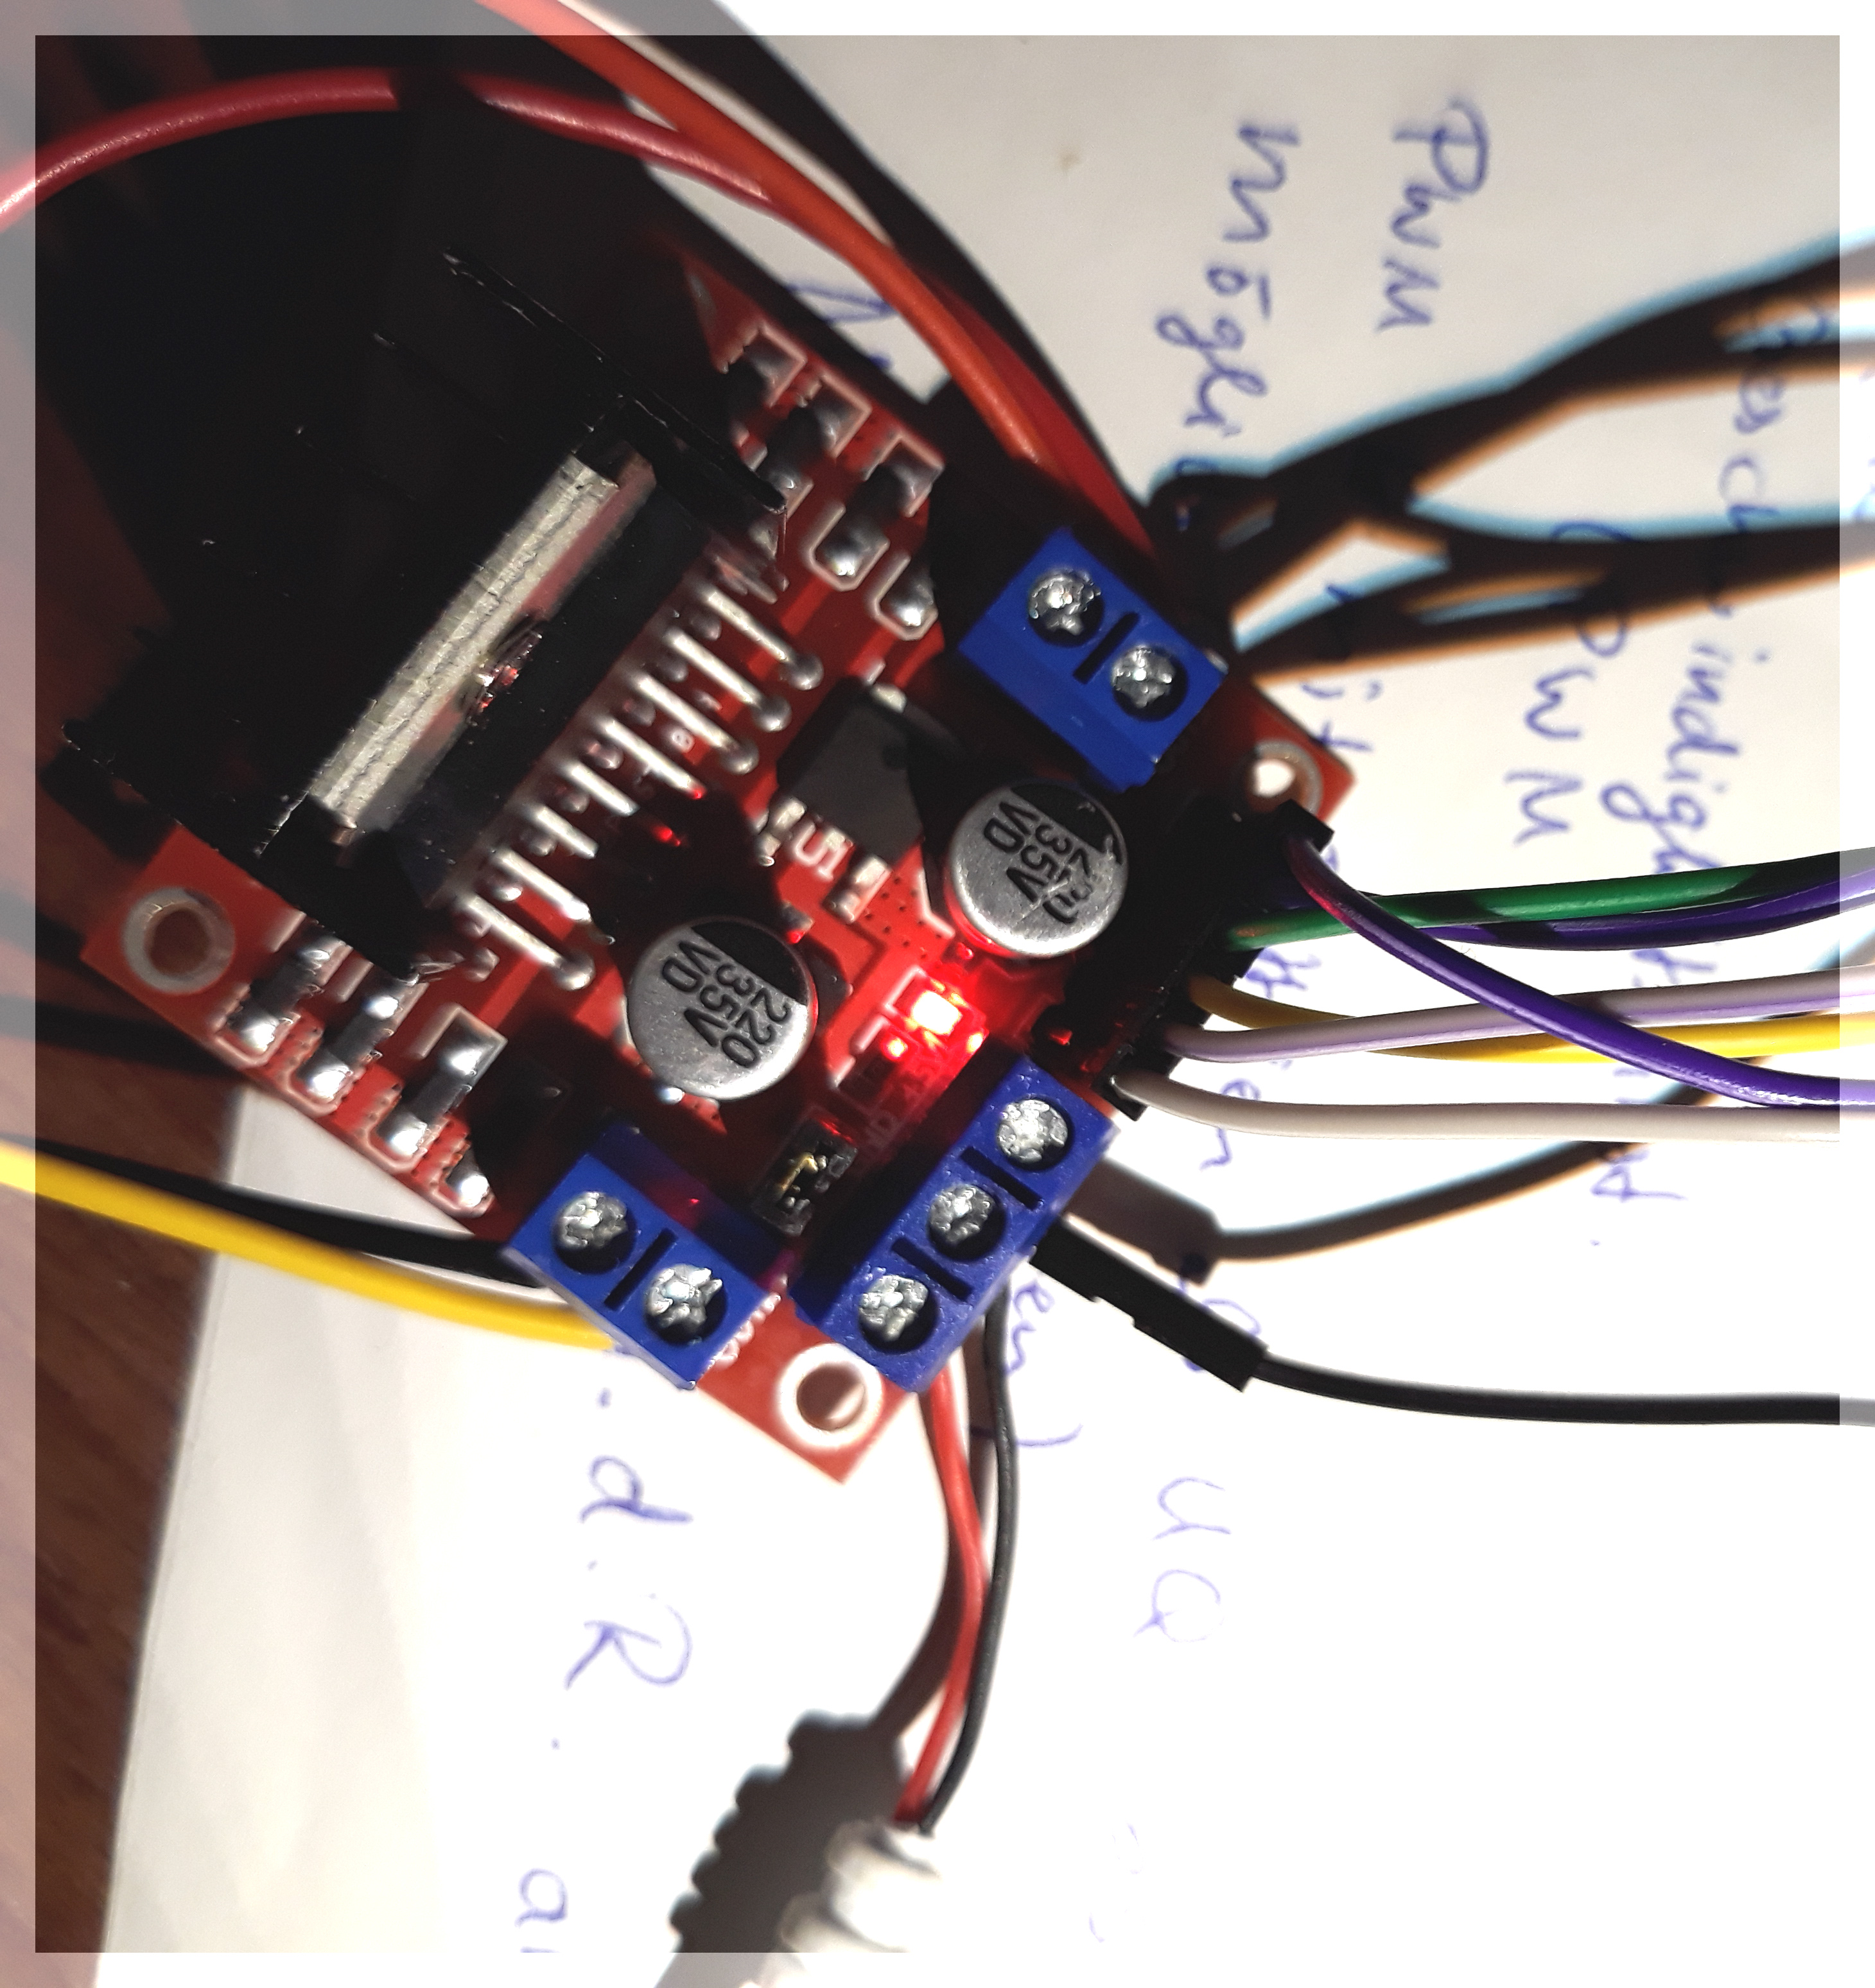
\includegraphics[width=5cm]{treiber_kabel.jpg}
\end{figure}

\begin{figure}[h]
\centering
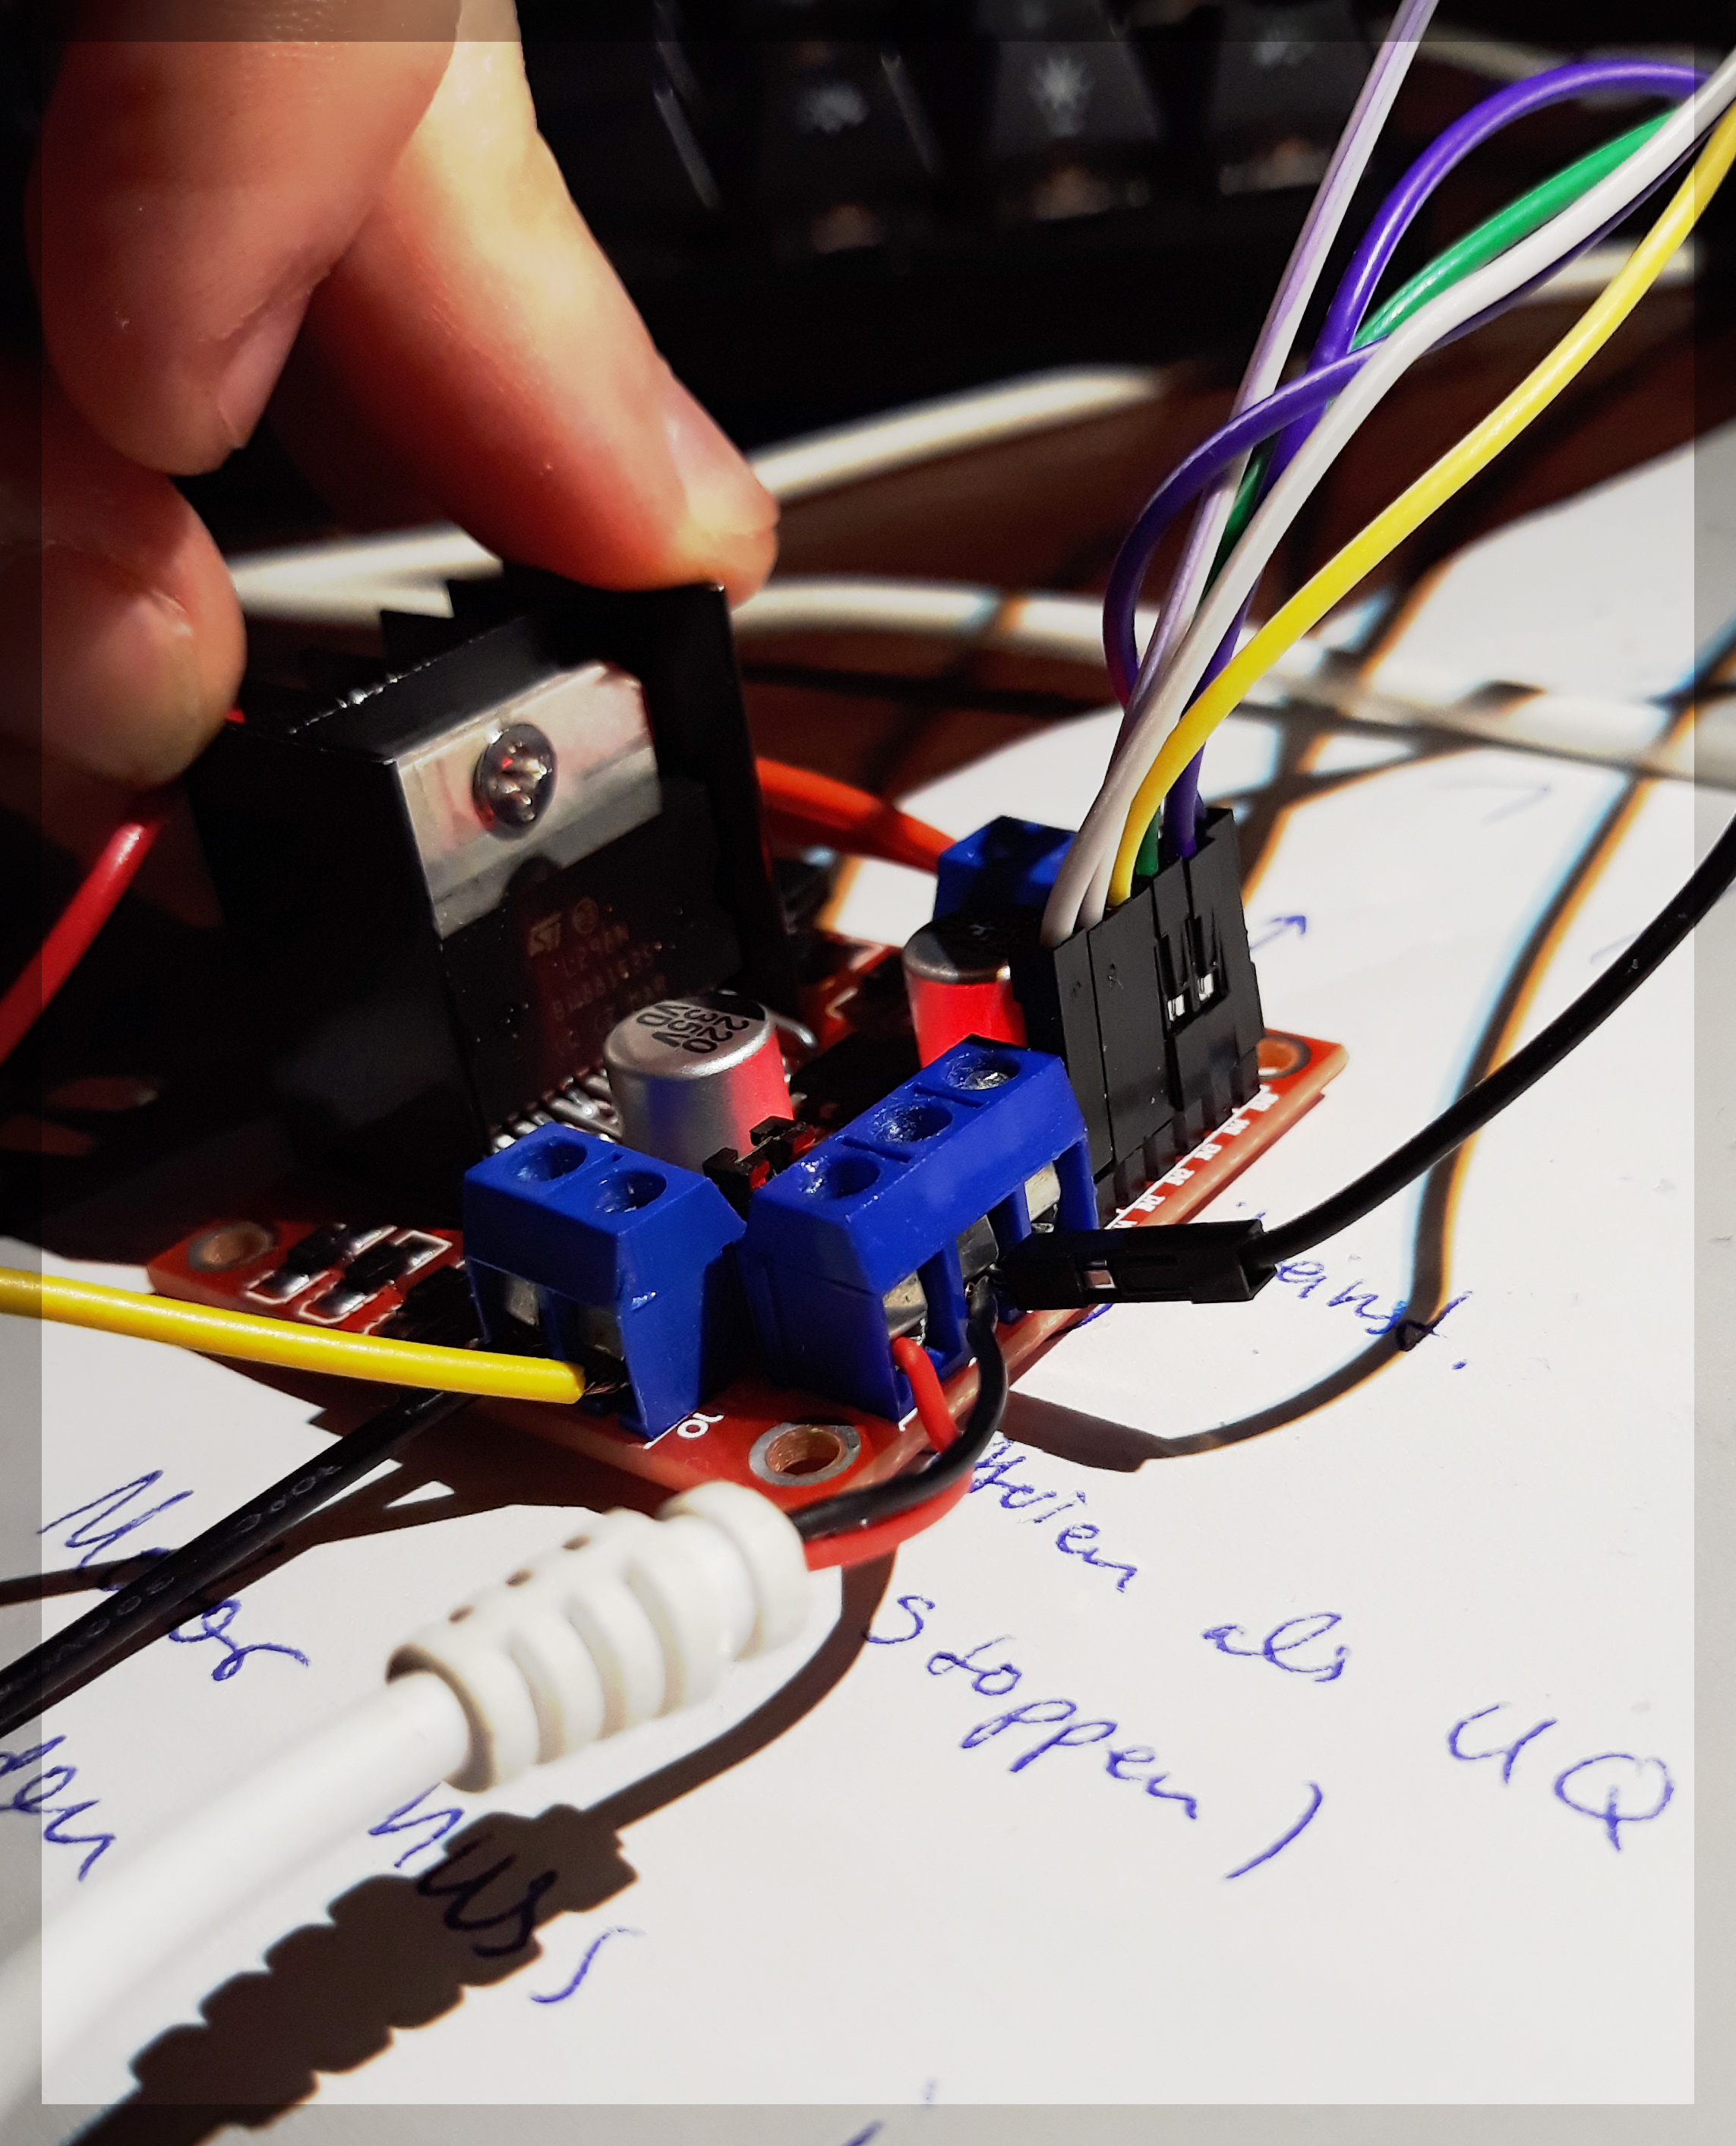
\includegraphics[width=5cm]{treiber_anschluss_close.jpg}
\end{figure}


Verbinden Sie den Raspberry Pi mit dem Motor sowie den Motor mit dem Treiber nach den Folgenden Tabellen.
Für die Verbindungen an den Klemmen öffnen Sie diese mit einem Schraubenzieher, schieben das Kabel hinein und schrauben sie fest. Für die Verbindungen an den Pins verwenden Sie steckbare Jumperkabel (Female to Female).\\

\schritt{1}{Verbindung der Motoren mit dem Treiber}{}
\begin{table}[h]
  \begin{center}
\begin{tabular}{@{}cc@{}}
\toprule
Motortreiber L298 & 12V Spannungsquelle \\ \midrule
OUT1              & Motor1(+)           \\
OUT2              & Motor1(-)           \\
OUT3              & Motor2(+)           \\
OUT4              & Motor2(-)           \\ \bottomrule
\end{tabular}
\end{center}
\caption{Verbindungen zwischen dem Treiber und den Motoren. Die Polarität der Motoren spielt keine Rolle.}
\end{table}


\schritt{2}{Verbindung des Treibers mit dem Raspberry Pi}{}

\begin{table}[h]
 \begin{center}
\begin{tabular}{@{}cc@{}}
\toprule
Raspberry Pi GPIO                                                & Motortreiber L298                                                                                                                               \\ \midrule
GPIO 20                                                          & IN1                                                                                                                                             \\
GPIO 16                                                          & IN2                                                                                                                                             \\
GPIO 19                                                          & IN3                                                                                                                                             \\
GPIO 4                                                           & IN4                                                                                                                                             \\
GPIO 12                                                          & ENA                                                                                                                                             \\
GPIO 13                                                          & ENB                                                                                                                                             \\
\begin{tabular}[c]{@{}c@{}}Masse (GND)\\ z.B. Pin 6\end{tabular} & \begin{tabular}[c]{@{}c@{}}Masse (GND) - Klemme\\ die selbe Klemme, an die auch (-)\\ der Versorgungsspannung angeschlossen\\ wird\end{tabular} \\ \bottomrule
\end{tabular}
\end{center}
\caption{Verbindungen zwischen dem Raspberry Pi und dem Motortreiber. Die Bezeichnungen des Treibers stehen auf der Board-Ober- oder Unterseite}
\end{table}

Die letzte Verbindung in der Tabelle sollte beachtet werden! Es bietet sich an, sie mit einem Male-to-Female Jumperkabel zu verbinden, wie im Bild oben sichtbar.\\

\schritt{3}{Verbindung der Versorgungsspannung an den Treiber}{}
Für diese Verbindung eignet sich ein Adapter, der den Stecker des 12V Netzteiles auf zwei einfache Kabel führt, um diese an die Klemmen des Treibers anzuschließen.

% Please add the following required packages to your document preamble:
% \usepackage{booktabs}
\begin{table}[h]
  \begin{center}
\begin{tabular}{@{}cc@{}}
\toprule
Motortreiber L298 & 12V Spannungsquelle          \\ \midrule
+12V              & +12V (i.d.R. rotes Kabel)    \\
GND               & GND (i.d.R. schwarzes Kabel) \\ \bottomrule
\end{tabular}
\end{center}
\caption{Verbindungen zwischen Treiber und Netzteil}
\end{table}


\subsection{Programmierung}
\subsection{Programm A (Beispiel)}
\subsection{Programm B}
